% This version uses the latex2e styles, not the very ancient 2.09 stuff.
\documentclass[letterpaper,twocolumn,11pt]{article}
\usepackage{usenix,epsfig,endnotes}
\usepackage{hyperref}
\usepackage{framed}
\usepackage{caption}
\usepackage{float}
\usepackage{amsmath}



\begin{document}

%don't want date printed
\date{\today}

%make title bold and 14 pt font (Latex default is non-bold, 16 pt)
\title{\Large \bf  Link Prediction in Bipartite Networks}

%for single author (just remove % characters)
\author{
{\rm Anirudh Narasimhamurthy}\\
u0941400\\ 
University Of Utah
\and
{\rm Soumya Smruti Mishra}\\
u0926085\\ 
University Of Utah
% copy the following lines to add more authors
% \and
% {\rm Name}\\
%Name Institution
} % end author

\maketitle

% Use the following at camera-ready time to suppress page numbers.

\thispagestyle{empty}

\subsection*{Abstract}
One of the challenges in network analysis is to predict what new connections will be created in the particular graph/network at some point in future. Many real world networks like user-products or user-business relations have a bipartite nature to them and evolve during time. Predicting links that will appear in them is one of the main approaches to understanding them. This was our main point of interest and we decided to understand link prediction problem in bipartite networks in our project. We also see how this can be extended or formulated to be applied to a recommendation problem. 


\subsection*{Classification Keywords}
link prediction, collaborative filtering, recommendation, bipartite graph,


\section{Motivation}
The primary motivation for selecting this project was based on two reasons: 
\begin{enumerate}
\item Firstly we wanted to explore and learn about link prediction and bipartite graphs. From our literature survey and reading papers \cite{two} \cite{six} \cite{seven} \cite{eight} we realized that link prediction in bipartite graphs was something which was less explored and hence we were interested to learn more about it through our project. 
\item Secondly we were also trying to see if we could use any of the Machine Learning techniques which we had learned about in this project and we believed the problem which we chose would probably help us in achieving it. 
\end{enumerate}

\section{Introduction}

\begin{itemize}
\item[] Link prediction is an important research problem in dynamic network analysis. Most of the problems which can be modeled as networks today are dynamic in nature i.e they evolve with node and link additions and removals. Typical examples include user - product relations where users are linked to the products they bought.


\item[] \cite{nine} states that social networks are not static and keep growing with time with addition of new nodes and links. Similarly user-product networks also evolve with time. This deals with link formation in the graphs i.e given nodes in a network the network grows by forming new relationships with existing nodes. We in this project deal with the question of predicting if a link will be formed between user and product/business.


\item[] Being able to predict such links accurately can have important implications in different networks including uses in national defense, predicting future credit card frauds and other related problems.Also a lot of the current research from what we understood focuses on link prediction on graphs with one type of node such as predicting links in social networks(Twitter, Facebook, LinkedIn) which is made up of people only. We wanted to explore methods which could be applied for a bipartite graph setting.


\item[] In this project we attempted to use our understanding of the concepts we learned in this course in line with different methods we came across the literature and used the following methods for link prediction in bipartite graph:
\begin{enumerate}
\item Similarity measures using Jaccard similarity and common neighbors
\item Approach based on completing the matrix entries using SVD
\item A page rank style approach using Random walks.
\item Supervised binary classification method.
\end{enumerate}
\end{itemize}

%After a new question is submitted in stackoverflow, most of them turn out to be invalid questions which are closed due to one of the following reasons: Off topic, not constructive, not a real question, too localized or exact duplicate. Hence, Kaggle posted a competition to use machine learning strategies to identify the best prediction model.

%
%\begin{figure}[H]
%\begin{center}
%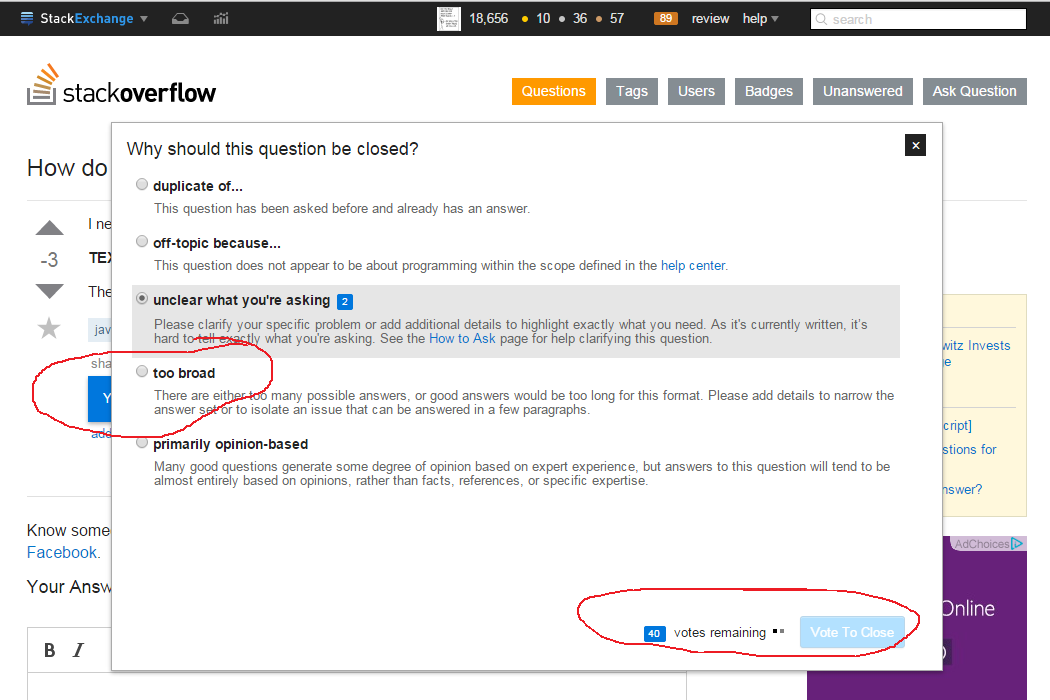
\includegraphics[width=1\linewidth]{labels.png}
%\captionof{figure}{Labels generated by Stack overflow for closed questions}
%\label{fig:status}
%\end{center}
%\end{figure}
%

\section{Formal Problem Description}

Our project attempts to predict new links which can potentially be formed in a network in future, given a snapshot of the current network and to evaluate its effectiveness. We are also primarily involved in applying the different metric to bipartite graphs.


\section{Definitions}
Bipartite graph: A bipartite graph or bigraph is a set of graph vertices decomposed into two disjoint sets such that no two graph vertices within the same set are adjacent to each other.

\section{Assumptions}
\label{sec:assumptions}
\begin{enumerate}
\item One of the primary assumptions that we make is although collaborative filtering recommendation technique might work with the data set, our interest was to learn about link prediction in bipartite graphs and so we model our data set as bipartite graph.
\item Link prediction is our primary goal and recommendation is a side product of this one and we assume the recommendation or result which we state in our later sections might be a possible result although the sparsity and other factors might point otherwise.
\item Also for our data set without taking the location into consideration, we assume the prediction that we make is reasonable one although in practice there could be a lot of other things needed to make such a prediction.
\end{enumerate}

\section{Scope}

Our main stating is that the approaches used in our project could potentially be applied to a different data set which exists as or can be modeled as bipartite graph and even if the example data set which we have taken might not sufficiently convince that, we wanted to make it clear that our scope lies in the understanding of methods/measures which could be applied for link prediction in bipartite graphs. Results and other observations stated in later sections are our understanding but the bigger picture could or could not be different. 

\section{Prior Work}

\begin{itemize}

\item[] A lot of work has been done on link prediction in general.In \cite{four} they experiment with several similarity metrics including Graph Distance, Preferential attachment, Katz method and others. These could be modified so that they can be applied to bipartite graphs. In our project we experiment with two similarity metrics stated in Introduction section.

\item[] 

\end{itemize}

\section{Dataset and features used}

\subsection{Major Dataset used for results}
StackOverflow Dataset:\\
Schema explained: 

\subsection{Dataset creation}
We planned to solve a supervised learning problem.
Since the problem invovled was a part of the Kaggle data competition, Kaggle had its own test dataset which it did not make it publically available. Hence we split the  initial training dataset \cite{stackdataset} (178351 examples) by random sampling into training and test datasets with size of dataset in the ratio 8:2 respectively so that we could evaluate the accuracy of our classifier against the test data.
We didn't look at the test data set until the evaluation part.

\subsection{Real valued features modification}
The features, which have real values, were grouped in two ranges: the values above the median were mapped to a value 1 and the values which were below the median were mapped to a value -1.

%\subsection{Derived Features creation}
\subsection{Baselined features}
Kaggle had provided a basline model for this problem. It had six features from the dataset to represent each post on the network as a vector of features. The six features are listed below alongwith a short explanation of their importance:
\begin{enumerate}
	\item \textbf{OwnerUndeletedanswersAtPostCreation:}count of answers posts the user had made that were undeleted when that row?s question was submitted
	\item \textbf{BodyLength:} This is the initial body length including
its code blocks lenth.
	\item \textbf{ReputationAtPostCreation:}User reputation at  post creation time.
	\item \textbf{NumTags:}Number of tags that the assigns to the post. Its maximum value is 5 per post.
	\item \textbf{TitleLength:}Title length of the post.
    \item \textbf{AgeofPost:} The difference in days between the system date and post creation date.
\end{enumerate}

These baselined features do not take into account the context of the post. Apart from the baselined features, information about the user was also available. The user information could also be related to the fact if a question will be closed or not. For instance if the user who had posted a question is a relatively new member and if the baselined feature values are relatively low, then chances are that the question posted by him might be predicted as one of Off-Topic, Not Constructive, Not a Real Question or Too Localized.

\subsection{Post features}

The actual post made on the site contains several meta data information. The text in the post could be represented as a vector using the tf-idf-weight technique or the Latent  Dirichlet Allocation(LDA). We did not explore on the text features as the baselined feature did not have them and also it involved some amount of work, which we could have implemented had we had more time to run our experiments. Some of the important features from the post which is used in our prediction are provided below:

\begin{enumerate}
    \item \textbf{CBCount:}Number of code blocks in the post?s body.
    \item \textbf{LinkCount:}Number of links in the post?s body
    \item \textbf{NumberOfDigits:} Number of digits in the post's body.
    \item \textbf{NumberOfSentences:}Number of sentences in the post
body excluding code blocks.
    \item NumberOfSentencesStartsWithI
    \item \textbf{NumberOfSentencesStartsWithYou:} Number of Sentences in the post which start with ?you?.  Referring to different literature gave us the information that conversational questions are more often
directed at readers by using word ?you?, while informational questions are more often focused on the asker by using the word ?I?
    \item UpperTextLowerTextRatio
    \item \textbf{FirstTextLineLength:}Length  of  the  first  text  line. Usually first short line implies personal appeal or greeting. The former case is the most interesting if it is peculiar to one of the close categories.
    \item NumberOfInterrogativeWords
    \item \textbf{NumberOfSentencesStartsWithInterrWords:}  Number of  sentences  which  starts  with  interrogative  words. This gives us an idea or information on whether the post is a question or not.

\end{enumerate}

%\subsection{Tag features}
%
%Every question posted on Stackoverflow must be tagged with atleast one tag. The dataset also had five features for the tags namely
%\begin{enumerate}
%	\item Tag1
%    \item Tag2
%    \item Tag3
%    \item Tag4
%    \item Tag5
%\end{enumerate}    

%During classification, we counted frequencies for  each  tag  and  each  category. We also counted frequencies  for  every  tag  pair. The  reason behind is that tags reflect some topics of the post.A pairwise occurrence of some tags can mean that two topics that lead to disputes may occur in one post.

\subsection{Training and test examples information}


\begin{table}[h]
	\centering
	\begin{tabular}{ |p{4cm}|p{2cm} |}
		\hline
		Training examples count		&	142681\\  \hline
		Test examples count &	35670 \\  \hline
		
	\end{tabular}
	\caption{Training and test examples count} 
	\label{tab:dist1} 
\end{table} 


%\subsection{Distribution of examples for each label on the entire dataset:}
%Refer ~\ref{tab:dist} for the distribution.

\begin{table}[ht]
	\begin{tabular}{ |p{3.5cm}|p{3.5cm} |}
		\hline
		\textbf {Label} & \textbf{Number of examples}\\ \hline
		Open		&	89337\\  \hline
		Not a Real Question	&	38622 \\  \hline
		Not Constructive	&	20897 \\  \hline
		Off Topic		&	20865\\  \hline
		Too Localized		&	8910\\  \hline
		
	\end{tabular}
	\caption{Distribution of training examples for each label on the total dataset (test +train)} 
	\label{tab:dist} 
\end{table} 


\section{Vowpal wabbit and scikit}

\subsection{SVM using Vowpal Wabbit}
Vowpal Wabbit (VW) \cite{vowpalwabbitwiki} is a library and algorithms developed at Yahoo! Research by John Langford. VW focuses on  the  approach  to  stream  the  examples  to  an  online-learning algorithm compared to the batch setting over many machines. As stated earlier we tried to compare the performance of vowpal wabbit and our classifier. We installed vowpal wabbit and implemented the SVM model

Vowpal Wabbit creates a model.vw after training with train data set. vw refers to vowpal wabbit extension. A csv to vw python program was also coded for this purpose since the input data was in csv format. After feeding the test data to the model, it creates a predictions dump for each example as shown in the figure ~\ref{fig:vw}. Refer ~\ref{tab:accuracy} for the accuracy obtained.

\begin{figure}[H]
\begin{center}
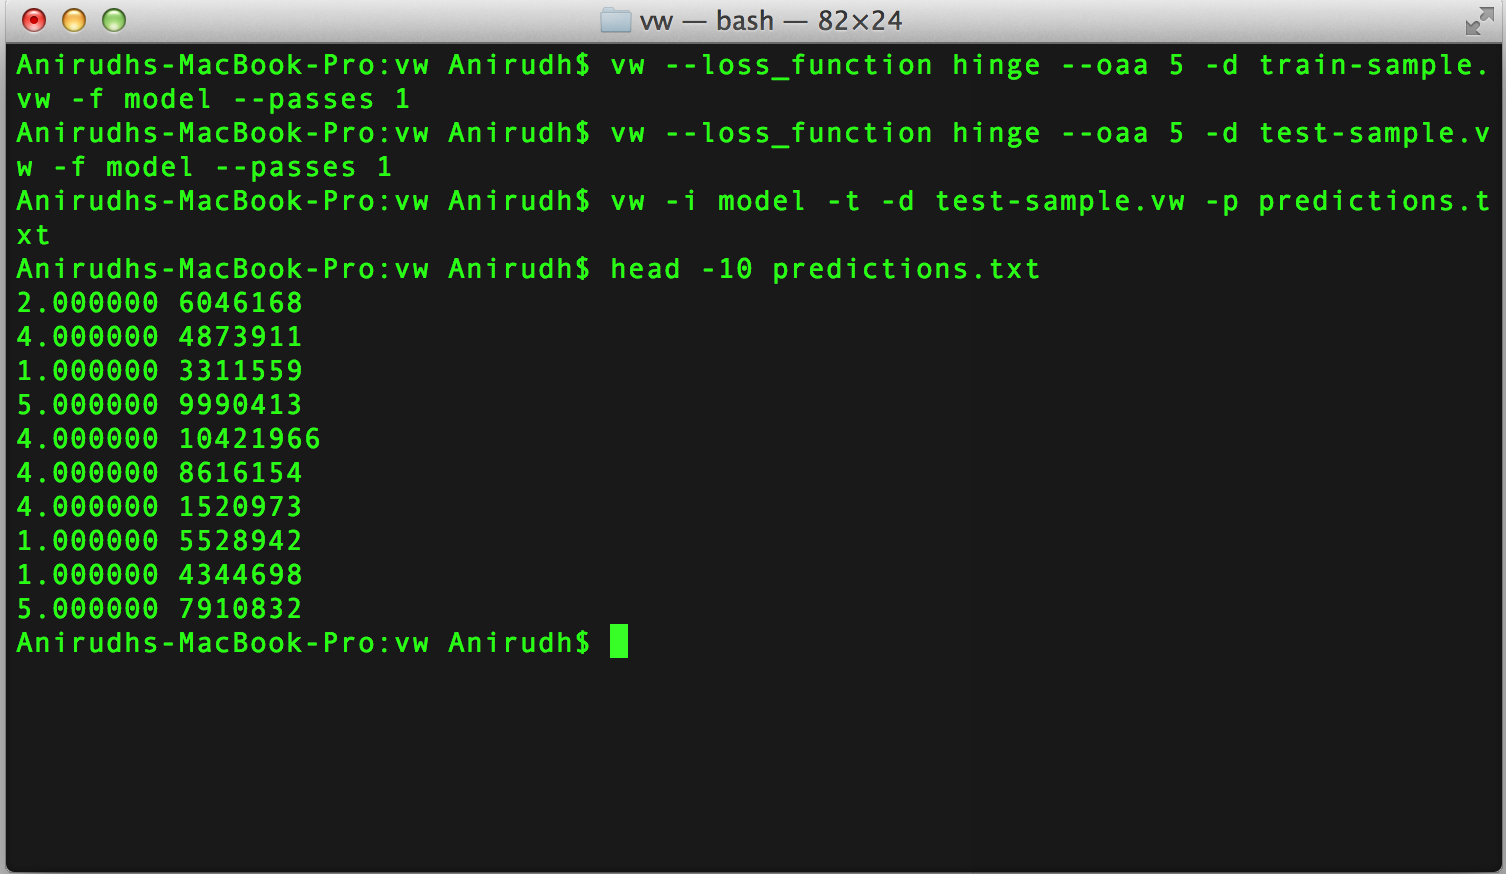
\includegraphics[width=1\linewidth]{vw.png}
\captionof{figure}{Vowpal Wabbit(VW) predictions using SVM}
\label{fig:vw}
\end{center}
\end{figure}

\subsection{Random Forest(RF) using scikit}
scikit provides a very rich library sklearn.ensemble.RandomForestClassifier which was easy to use to build a random forest for our given dataset. Refer ~\ref{tab:accuracy} for the accuracy obtained.

\section{Custom implementation}

In this section we descibe our implementation of the different models and also their accuracies.

\subsection{Ideas used from the class/course material}
%What ideas from the class did you use?
%What are the important ideas you explored?
We wanted to model our problem to be a multi-class classification problem. Also having gone through different literature and considering the coding and effort involved, we decided to use one vs all decomposition technique as opposed to all vs all technique.

On a lighter note, we performed cross-validation for selecting the decomposition technique by checking out the technique used by the top 10 finisher of this Kaggle problem contest and we probed on ideas on the below methods:
\begin{enumerate}
\itemsep0em
\item Random forest using bagging \& one vs all.
\item SVM using SGD \& one vs all.
\item Ensembles of Decision trees \& one vs all.
\end{enumerate}

\subsubsection{Multiclass classification one vs all}
In this problem we have five labels (open,OT,NC,NRQ,TL), hence we would have 5 decision trees (or) 5 SVM models if we were to build the multi-class classifier using our existing binary classifiers.For instance, Labels OT and the complement $\overline{OT}$ are decided by one of the models. Similarly, there would 4 other models. 

Hence, we would use 5 binary classification methods to achieve multiclass classification for prediction of the status of each post.

The final predicted label corresponding to max value of the $H_{final}$ would be final prediction using one vs all decomposition.

\subsubsection{Random forest using bagging \& one vs all}

We developed upon our class homework and we randomly sampled examples with replacement and created 5 data sets. We created decision trees for each of the 5 data sets as indicated in \cite{rfwiki}. That is the decision trees had only a subset of the total features available for the children.

After creation of such decision trees, final predicted label for any test example would be based on majority vote from these 5 decision trees. Then, as usual one vs all will be applied with majority vote as well.

\subsubsection{SVM using SGD \& one vs all}
Similar to the above model, we created 5 SVM models for each of the labels. For instance, OT and $\overline{OT}$ would have a SVM model.Each of the models had a weight vector.

The final prediction for any example was the label corresponding to max value of wx. Stochastic Gradient Descent algorithm was used and the regularizer used in objective function in our implementation was C=1. Since we are in the online setting and fitting in all the examples at once wasn't necessarily good, stochastic gradient descent worked well by taking on example at a time and developed the prediction model.

\subsubsection{Ensembles of Boosted Decision trees \& one vs all}
We performed 5-fold cross-validation on training data. Boosting based on decision trees was harder than expected. We need to boost the examples which were misclassified, but our feature values were -1s and 1s. Hence, boosting or penalizing 1 or -1 is not possible respectively. This was not done primarily because of the fact that the complexity of the decision trees would increase as feature space.

We have partially implemented this since this suggestion was given in the intermediate report, but we couldn't eventually complete the suggested idea due to the above reason. 

\section{Ideas Explored but not used}
This section describes some of the ideas which we brainstormed and further wanted to explore. Although both of us couldn't concur with the views and validity of the idea proposed, we thought it would be good to mention it here:
\subsection{Combination of SVM and Decision Tree}
\begin{enumerate}
\itemsep0em
\item We would know the prediction label for each example from each of the methods - SVM and RF.
\item We could consider the prediction values from the 4 methods  as feature vectors.
\item Final prediction label for a example x would correspond to the label with higher wx, where w is the normalized prediction accuracy of that particular model
\item Say accuracy of the methods 1,2,3,4 are a1,a2,a3,a4. Then the w1=a1/(a1+a2+a3+a4)
\item But this model was purely \textbf{based on intuition}, we didn't have enough proof to assume so.Hence we discarded implementation of this model.
\end{enumerate}


\section{Evaluation of test dataset}
%Results (or for theoretical project, proofs)

We executed each test example in the models above. The final accuracies are tabulated. Refer ~\ref{tab:accuracy} for the accuracy of each method.

\begin{table*}[ht] 
\centering
\begin{tabular}{ |p{4.5cm}|p{3cm} |}
\hline
\textbf{Methods} & \textbf{Accuracy}\\ \hline
SVM using vowpal wabbit	&	67.03  \\  \hline
RF using scikit	&	64.58  \\  \hline
Custom SVM using SGD one vs all &  61.96  \\  \hline
Custom RF (Bagging of Decision tree) one vs all &  59.19  \\  \hline
\end{tabular}
\caption{Accuracies for multiclass classification} 
\label{tab:accuracy} 
\end{table*} 

As per paper\cite{DBLP:journals/corr/CorreaS13}, prediction based on both user and post datasets was 73%.

\subsection{Inference about the result}
%What did you learn?
AgeofPost, CBCount - number of code blocks, Reputation at post creation date and BodyLength-length of the post were the most relevant features. Most of the decision trees created for bagging had these 4 features in common. SVM weight vector values for these 4 features were among the top 5 as well. Reasoning about this higher weights would give the intuition that higher the weight more it will contribute to the argmax for one vs all.


\section{Conclusion}
The features used which were based on the posts, tags and user information did a decent enough job for the prediction model. The baselined features were slightly limited, coming to think of it in broader perspective and some more additional features or other derived features which could have been obtained from the user and post data could have improved the accuracies of our model. 

We see that the vowpal wabbit implementation did relatively better than our model but the fact that we were able to implement a basic multi-class classification was satisfying. Also the performance provided by scikit for the random forests was also slightly better because of the internally optimized python code. 

Additionally the text sentiment analysis and text comparison in stack overflow database would lead to better results in prediction of whether a stack overflow question will be closed. This is mainly because the content of the question plays a very important role in the diagnosis of whether the question will be closed.

In conclusion we were able to build a multi-class classifier which could predict the status of a question on StackOverflow and the results could be used to then determine if the question should be closed or not.

\section{Difficulties faced in implementation}
\begin{enumerate}
\itemsep0em
\item First and foremost, we needed to preprocess the data for vowpal wabbit in vw format.
\item We faced too many installation issues for Vowpal wabbit. We didn't have a clear man page for commands to be used unlike scikit.
\item We also needed to preprocess data for custom implementations.
\item Since we implemented bagging(ensemble) of decision trees for class homeworks, - Custom RF (Bagging of Decision tree) One Vs all was relatively easy.
\item Custom SVM One vs All implementation involved creating SVM model objects for each hypothesis similar to Custom RF.
\end{enumerate}


\section{Future Work}
%If you had much more time, how would you continue the project?

\begin{itemize}
\itemsep0em
\item We assumed 0 or 1 for real valued features for ease of implementation, which could be improved to include more values to increase accuracy of prediction.
\item Due to time crunch, we were not able to increase the number of random sub-samples selected for random forest.
\item We could easily find out the link to related user data set, which is not available now. If we had the link, the our prediction accuracies might have been closer to the paper \cite{Lezina_predictclosed}.
\item  The text in the post could be represented as a vector using the tf-idf-weight technique or the Latent  Dirichlet Allocation(LDA). We could explore more on this.
\item While brainstorming, we had seen combinations of Decision Tree and SVM method called DTSVM in the paper\cite{5695459}. DTSVM is a faster algorithm which produces equivalently good prediction accuracies.
\end{itemize}



\bibliographystyle{plain}
\begin{thebibliography}{100}
	\bibitem{one} Lars Backstrom , Jure Leskovec, Supervised random walks: predicting and recommending links in social networks, Proceedings of the fourth ACM international conference on Web search and data mining, February 09-12, 2011, Hong Kong, China.   
    \bibitem{two} J. Kunegis, E. De Luca, and S. Albayrak. The link prediction problem in bipartite networks. In Computational Intelligence for Knowledge-Based Systems Design. 2010.
	\bibitem{three} Y. Yamanishi. Supervised bipartite graph inference. In NIPS, D. Koller, D. Schuurmans, Y.Bengio, and L. Bottou, Eds. MIT Press, 2008, pp. 18411848.
    
    \bibitem{four} Liben-Nowell, David and Kleinberg, Jon, The link-prediction problem for social networks,Journal of the American Society for Information Science and Technology,http://dx.doi.org/10.1002/asi.20591,2007.

    \bibitem{five} N. Benchettara, R. Kanawati, C. Rouveirol. Supervised Machine Learning applied to Link Prediction in Bipartite Social Networks. In Proceedings of the International Conference on Advances in Social Network Analysis and Mining. IEEE, Los Alamitos, CA, 326-330, 2010
    
   \bibitem{six} O. Allali, C. Magnien and M. Latapy , "Link prediction in bipartite graphs using internal links and weighted projection" ,  NetSciCom , pp.953 -958 
   
   \bibitem{seven} Xin Li , Hsinchun Chen, Recommendation as link prediction: a graph kernel-based machine learning approach, Proceedings of the 9th ACM/IEEE-CS joint conference on Digital libraries, June 15-19, 2009, Austin, TX, USA
   
   \bibitem{eight} Zan Huang , Xin Li , Hsinchun Chen, Link prediction approach to collaborative filtering, Proceedings of the 5th ACM/IEEE-CS joint conference on Digital libraries, June 07-11, 2005, Denver, CO, USA 
    
    \bibitem{nine} https://www3.nd.edu/~dial/papers/ICDM12b.pdf
    
\end{thebibliography}


%
%
%
%{
%\small 
%\bibliographystyle{acm}
%\bibliography{report}
%}

\end{document}